% !TEX root = _yoko.tex

% ==========================================
% プロジェクト予稿（1P）の本文
% ==========================================

\section{はじめに}

筆者は 10 年来「NEWS」というアイドルグループ
を応援し続けており，彼らを応援している中で
「NEWS は背中を押してくれる楽曲が多い」という
声や，メンバーが「エモーショナルさが NEWS の魅
力になってきている」と発言を聞いていた．
そこでNEWS 楽曲の歌詞の特徴に着目し，歌詞傾向につい
て考察を行い楽曲のどういう点から「エモーショナルさ」
や「背中を押された」と感じるのか分析することを目的としている．


\section{対象楽曲とデータ形成}
本研究の分析に際し，収集する必要のあるデータは「曲
名」「発売日」「歌詞」「グループ人数」の４つである．今回
分析対象とした NEWS 楽曲は，歌ネット \cite{utanet}に基づいて収
集した 266 曲 (2024/11/13 現在) である．

作成した歌詞データに対してKHcoder\cite{khcoder}を使用し，分析を進めるためのデータ形成を行った．
品詞ごとに集計し，回数とそれに対応する割合を求めている．
そしてリフレインに考慮し出現回数と使用曲数の２種類を求めた．

\section{対象楽曲とデータ形成}

2章で作成したデータをもとに各品詞の分析を行った．ここでは名詞の「夢」を例に取り上げる．
形成したデータをもとに「夢」の時代別使用頻度推移を出力した（図1）．

	\begin{figure}[b]
		\centering
		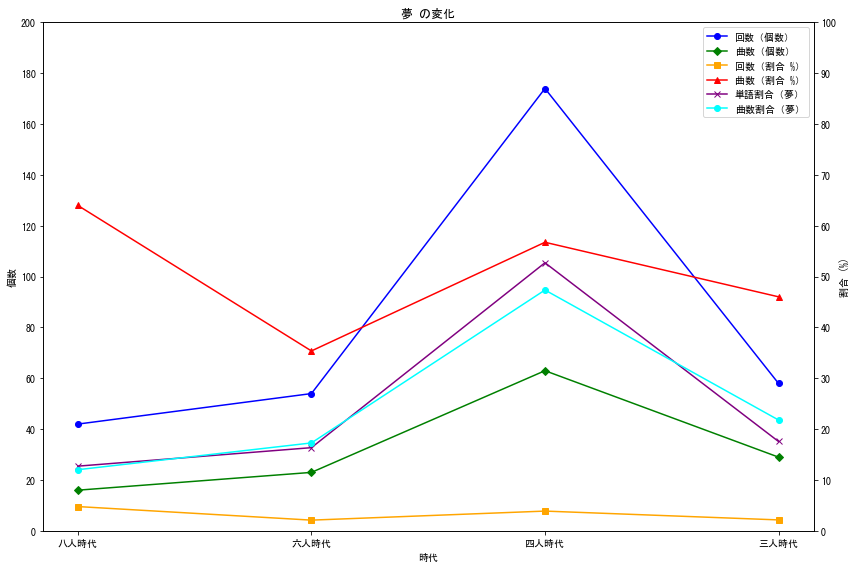
\includegraphics[width=\hsize]{fig/meishi-yume.png}
		%\subcaption{「夢」}
		\label{fig:yume}
\caption{「夢」の時代別使用頻度推移}
	\end{figure}

また，辞書での意味\cite{yume}を参考に単語をどのような意味で使用したのかについて人数ごとの比較グラフを出力した（図2）

\begin{figure}[tb]
		\centering
		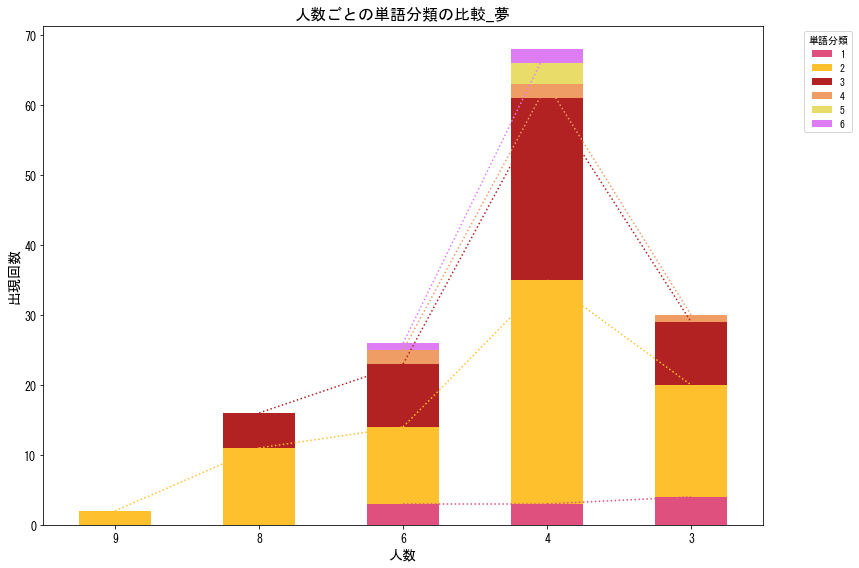
\includegraphics[width=\hsize]{fig/yume-ninzu.png}
		%\subcaption{「夢」}
		\label{fig:yume-ninzu}
\caption{「夢」の時代別使用意味比較}
	\end{figure}

\section{キーワードごとの分析}
NEWSにおいて「背中を押す」と「エモーショナルさ」をキーワードとして設定し，それに対応する楽曲をサンプルとして分析を行った．
以下は「背中を押す」NEWS楽曲をサンプルにし名詞の頻出単語上位10個を時系列累積グラフとして出力したものである（図３）．

\begin{table}[tb]
	\centering
	\caption{選曲した35曲の名詞出現回数上位10単語}
	\label{tab:news-senaka}
	\begin{tabular}{cc|cc}
		\hline
		単語 & 出現回数 & 単語 & 出現回数 \\ \hline
		夢  & 79     & 空  & 30     \\
		自分 & 54     & 笑顔 & 26     \\
		未来 & 35     & 胸  & 23     \\
		涙  & 34     & 声  & 22     \\
		心  & 32     & 道  & 20     \\
		\hline

		%「表の中身を書く」
	\end{tabular}

\end{table}

\begin{figure}[tb]
	\centering
	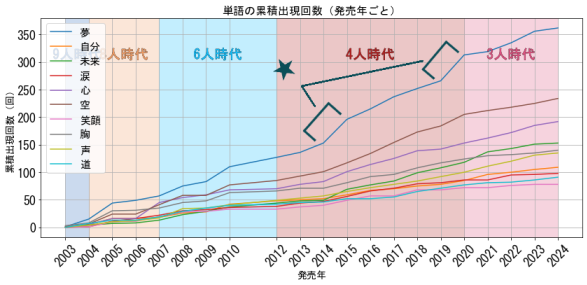
\includegraphics[width=\hsize]{fig/top10-news-senaka-ruiseki.png}
	\caption{表１をもとに全楽曲を対象とした単語の累積グラフ}
	\label{fig:top10-news-senaka-ruiseki}
	\end{figure}

\section{まとめ}

出力結果からNEWSの楽曲はとある時期を境に単語が増加する傾向が見られた．
今回は歌詞にのみ着目したが，メロディなどほかの要素を加えることでより詳しい分析になるだろう．
